\documentclass[a4paper,twosided,11pt,DIV14]{scrartcl}
%
% all the local settings defined in /localsettings.sty
\usepackage{localsettings}
\usepackage{customsymbols}
%
% lazyeqn - math symbols
% Uncomment if you have chosen to clone it to your project
\usepackage{./lazyeqn/lazyeqn}
\addtokomafont{disposition}{\rmfamily}
%
\usepackage{scalefnt}

\newcommand\smallerr[2][0.85]{{\scalefont{#1}#2}}

\newcommand\ilabel[1]{I\smallerr{#1}}
% \usepackage{accents}

% \newcommand\ub[1]{%
%   \underaccent{\bar}{#1}}

% \makeatletter
% \def\ub#1{\underline{\sbox\tw@{$#1$}\dp\tw@\z@\box\tw@}}
% \makeatother

\DeclareMathOperator{\ivt}{ivt}
\DeclareMathOperator{\idxop}{idx}
\DeclareMathOperator{\per}{per}
\DeclareMathOperator{\rank}{rank}
\DeclareMathOperator{\ifop}{if}
\DeclareMathOperator{\invop}{inv}

% \makeatletter
% \newcommand{\idxop}{\mathop{\operator@font idx}}
% \newcommand{\per}{\mathop{\operator@font per}}
% % \newcommand{\ivt}{\mathop{\operator@font ivt}}
% \newcommand{\rank}{\mathop{\operator@font rank}}
% \newcommand{\ifop}{\mathop{\operator@font if}}
% \newcommand{\invop}{\mathop{\operator@font inv}}
% \makeatother

\newcommand{\veps}{\vareps}

% \def\ub#1{\underline{\smash{#1}}}
\def\ub#1{\underline{#1}}

% \newcommand{\idx}[1]{#1_1 #1_2 \dotsm #1_N}
% \newcommand{\idxu}[1]{\ub{#1}_1 \ub{#1}_2 \dotsm \ub{#1}_N}
% \newcommand{\idxn}[2]{#1_1 #1_2 \dotsm #1_{#2}}
% \newcommand{\idxnu}[2]{\ub{\idxn{#1}{#2}}}

\newcommand{\idx}[1]{#1_1 \dotsm #1_N}
\newcommand{\idxu}[1]{\ub{#1}_1 \dotsm \ub{#1}_N}
\newcommand{\idxn}[2]{#1_1 \dotsm #1_{#2}}
\newcommand{\idxnu}[2]{\ub{\idxn{#1}{#2}}}

%
\frenchspacing
%
% \title{Array Calculus}
\title{Composites Modeling WS2014--2015\\Assignment}
\author{Hüseyin Onur Solmaz -- Matr.2868402}
\date{}
%



\begin{document}
\maketitle
\tableofcontents

\section{Introduction}

Composite materials used in the industry exhibit mechanical behavior that is
more complex than the ideal homogeneous materials we are familiar with from
elementary \emph{strength of materials} teachings. As a student of
Computational Mechanics of Materials and Structures, I felt compelled to take
this course, \emph{Composites Modeling}, which provided me insight on lots of
industrial areas of application.

In order to test our knowledge, this course required for us to finish a final
assignment, this one, which is supposed to allow us to demonstrate our
capabilities. The assignment consists of 5 tasks, which in order want us to
model a carbon-fiber and an epoxy-resin composite using micromechanics, laminate
analysis and FEM simulation. The results were compared for these different
approaches, using a common geometry and loading. After this, beads were added to
the geometry of the FEM simulation, and the strengthening effect was observed.
Finally, we were asked to model the RTM infusion process for the same given
geometry.

\section{Estimation of Material Constants (Task 1)}

\textit{The following tables give typical mechanical data for T300 carbon-fiber and
Hexcel 8551-7 epoxy resin.}

\begin{table}[H]
  \centering
  \begin{minipage}{0.45\textwidth}
    \footnotesize
  \begin{tabular}{p{0.7\textwidth}p{0.2\textwidth}}
    \toprule
    Fiber type & T300\\
    Longitudinal modulus $E_{1}$ (GPa) & 231\\
    Transverse modulus $E_{12}$ (GPa) & 15\\
    Transverse modulus $E_{13}$ (GPa) & 15\\
    In-plane shear modulus $G_{f12}$ (GPa) & 15\\
    Major Poisson's ratio $\nu_{f12}$ & 0.2\\
    Major Poisson's ratio $\nu_{f13}$ & 0.2\\
    Transverse shear modulus $G_{f23}$ (GPa) & 7\\
    Longitudinal tensile strength $X_{f1T}$ (MPa) & 2500\\
    Longitudinal compressive strength $X_{f1C}$ (MPa) & 2000\\
    Longitudinal tensile failure strain $\veps_{f1T}$ (\%) & 1.086\\
    Longitudinal compressive failure strain $\veps_{f1C}$ (\%) & 0.869\\
    \bottomrule
  \end{tabular}
  \end{minipage}
  \begin{minipage}{0.45\textwidth}
    \footnotesize
  \begin{tabular}{p{0.7\textwidth}p{0.2\textwidth}}
    \toprule
    Matrix type & 8551-7 epoxy\\
    Elastic modulus $E_{m}$ (GPa) & 4.08\\
    Elastic shear modulus $G_{m}$ (GPa) & 1.478\\
    Elastic Poisson's ratio $\nu_{m}$ (GPa) & 0.38\\
    Tensile strength $Y_{mT}$ (MPa) & 99\\
    Compressive strength $Y_{mC}$ (MPa) & 130\\
    Shear strength $S_{m}$ (MPa) & 57\\
    Tensile failure strain $\veps_{mT}$ (\%) & 4.4\\
    Compressive failure strain $\veps_{mC}$ (\%) & 9\\
    Shear failure strain $\gamma_{m}$ (\%) & 5.1\\
    \bottomrule
  \end{tabular}
  \end{minipage}
  \caption{Material parameters for the carbon-fibers (left) and epoxy resin
    matrix (right).}
\end{table}
\subsection{Estimation (Part a)}

\textit{Use necessary micro-mechanics formulae to estimate elastic modulus
  ($E_{1}$, $E_{2}$,
$G_{12}$), Poisson's ratios ($\nu_{12}$ and $\nu_{21}$) and failure properties for maximum stresses
($F_{1T}$, $F_{1C}$, $F_{2T}$, $F_{2C}$ and $F_{12}=F_{6}$) assuming the composite is unidirectional
with \textbf{a fiber volume ratio of 50\%}}
\subsubsection{Elastic and Shear Moduli}
%
$V_f$, the fiber volume fraction  is given to be $0.5$. The longitudinal
modulus $E_1$ for the \emph{Representative Volume Element} RVE is calculated as
%
\begin{equation}
  E_1 = E_fV_f + E_m (1-V_f)
\end{equation}
%
where $E_f$ and $E_m$ are the longitudinal moduli of the fibers and matrix
respectively. Using the formula, $E_1$ = \SI{117.54}{GPa}.
%
\\The inverse mixture relation is used for the transverse modulus $E_2$
%
\begin{equation}
  \frac{1}{E_2} = \frac{V_f}{E_{2f}} + \frac{V_m}{E_m}
  \eqor
  E_2 = \frac{E_{2f} E_m}{V_mE_{2f}+V_fE_m}
\end{equation}
%
where $E_{2f}$ is the transverse modulus of the fibers, and $V_m$ is the folume
fraction of the matrix. Using the formula, $E_2$ = \SI{6.415}{GPa}.
\\Similarly, the shear modulus is calculated as
%
\begin{equation}
  \frac{1}{G_{12}} = \frac{V_f}{G_{f12}} + \frac{V_m}{G_m}
  \eqor
  G_{12} = \frac{G_{f12} G_m}{V_mG_{f12}+V_fG_m}
\end{equation}
%
where $G_{f12}$ and $G_m$ are the shear moduli of the fibers and the matrix
respectively. Using the formula, $G_{12}$ = \SI{2.691}{GPa}.
%
\subsubsection{Hopkins-Chamis Model}
%
The Hopkins-Chamis model can be used to make a better estimate of $E_2$ and
$G_{12}$. It goes for $E_2$
%
\begin{equation}
  E_{2} = E_m\sbr{\sbr{1-\sqrt{V_f}}+\frac{\sqrt{V_f}}{1-\sqrt{V_f}\sbr{1-\frac{E_m}{E_{f2}}}}}
\end{equation}
%
yielding $E_2$ = \SI{7.141}{GPa}. Similarly $G_{12}$ = \SI{3.315}{GPa}.
%
These values will be used for all calculations.
%
%
\subsubsection{Poisson's Ratios}
%
Major and minor Poisson's ratios will be calculated following the same
principle, using direct and inverse mixture relations
%
\begin{gather}
  \nu_{12} = \nu_{f12} V_f + \nu_m V_m\\
  \frac{1}{\nu_{21}} = \frac{V_f}{\nu_{f21}} + \frac{V_m}{\nu_m}
  \eqor
  \nu_{21} = \frac{\nu_{f21} \nu_m}{V_m\nu_{f21}+V_f\nu_m}
\end{gather}
%
where $\nu_{12}$, $\nu_{21}$ and $\nu_m$ are the major and minor Poisson's
ratios and the Poisson ratio of the matrix respectively. Using the formulas,
$\nu_{12}$ = 0.290, $\nu_{21}$ = 0.262.
%
\subsubsection{Maximum Stresses}
\textbf{The failure stress at longitudinal tension} is calculated using the direct relation
%
\begin{equation}
  F_{1t} = \sigma_f V_f  + \sigma_m^{*} (1-V_f)
\end{equation}
where $\sigma_f$ is the longitudinal tensile strength of the
fibers and $\sigma_m^{*}$ is matrix stress at failure. The last one is
calculated as
\begin{equation}
  \sigma_m^{*} \approx \sigma_f \frac{E_m}{E_f}
\end{equation}
Using the formulas, $\sigma_m^{*}$ = \SI{44.156}{MPa} $F_{1t}$ = \SI{1272.1}{MPa}.
%
\\\textbf{The failure stress at transverse tension} is calculated as
%
\begin{equation}
  F_{2t} = E_{2} \veps_{2t\textsf{ult}}
\end{equation}
%
where $\veps_{2t\textsf{ult}}$ is the ultimate transverse strain at tension
%
\begin{equation}
  \veps_{2t\textsf{ult}} = \frac{\veps_{m\textsf{ult}}}{F}
\end{equation}
%
where $F$ is the \emph{stress concentration factor}
%
\begin{equation}
  F = \frac{\veps_m}{\veps_c} = \frac{1}{\frac{d}{s}\sbr{\frac{E_m}{E_f}-1}+1}
\end{equation}
%
Here $\frac{d}{s}$ is related to spatial configuration, and is equal to
$\sqrt{\frac{2}{\pi}}$. From this $F$ = 2.386.
$\veps_{m\textsf{ult}}$ is derived from the simple
relation
%
\begin{equation}
  Y_{mT} = E_m \veps_{m\textsf{ult}}
\end{equation}
and leads to $\veps_{m\textsf{ult}}$ = \num{24.265e-3} therefore $\veps_{2t\textsf{ult}}=$
\num{10.17e-3}. $F_{2t}$ is finally found out to be \SI{72.624}{MPa} using the
moduli obtained from Hopkins-Chamis model.
%
\\\textbf{The failure stress at longitudinal compression} is calculated for 3
different failure cases
\begin{enumerate}
\item For fiber micro-buckling,
  \begin{equation}
    F_{1c} = \frac{G_m}{1-V_f}
  \end{equation}
  and equals \SI{2956}{MPa}.

\item Transverse tensile rupture due to Poisson's effect
%
  \begin{equation}
    F_{1c} = \frac{E_{1}\veps_{2t\textsf{ult}}}{\nu_{12}}
  \end{equation}
  Using previously calculated values, \SI{4122}{MPa}.

\item Shear failure without buckling
%
  \begin{equation}
    F_{1c} =  2\rbr{\tau_{f\textsf{ult}}V_f + \tau_{m\textsf{ult}}V_m}
  \end{equation}
  where
    $\tau_{f\textsf{ult}} = \frac{\sigma_{\textsf{ult}}}{2}$ = \SI{1000}{MPa}
    and $\tau_{m\textsf{ult}}$ = \SI{57}{MPa} from given values. This yields
    \SI{1057}{MPa} for this case.
\end{enumerate}
%
%
\textbf{The failure stress at transverse compression} is calculated in the same
manner as transverse tension
%
\begin{equation}
  F_{2c} = E_{2} \veps_{2c\textsf{ult}}
\end{equation}
%
where $\veps_{2c\textsf{ult}}$ is the
%
\begin{equation}
  \veps_{2c\textsf{ult}} = \frac{\veps_{mc\textsf{ult}}}{F}
\end{equation}
%
where $F$ is the same stress concentration factor defined before and again
equals 2.386.
$\veps_{mc\textsf{ult}}$ is calculated similarly
%
\begin{equation}
  Y_{mC} = E_m \veps_{mc\textsf{ult}}
\end{equation}
and leads to $\veps_{mc\textsf{ult}}$ = \num{31.863e-3} therefore $\veps_{2c\textsf{ult}}=$
\num{13.354e-3}. $F_{2c}$ is finally found out to be \SI{95.361}{MPa}.
%
\\\textbf{The in-plane shear strength} is calculated as
%
\begin{equation}
  F_6 = F_{12} = G_{12}\gamma_{12}
\end{equation}
%
where
%
\begin{equation}
  \gamma_{12} = \frac{\gamma_{m\textsf{ult}12}}{F_s}
\end{equation}
%
where $\gamma_{m\textsf{ult}12}$ can be found from the relation
%
\begin{equation}
  S_m = G_m \gamma_{m\textsf{ult}12}
\end{equation}
%
and $F_s$ is the shear stress concentration factor defined as
%
\begin{equation}
  F_s = \frac{\gamma_{m12}}{\gamma_{c12}} = \frac{1}{\frac{d}{s}\sbr{\frac{E_{m12}}{E_{f12}}-1}+1}
\end{equation}
%
again, $\frac{d}{s}=\sqrt{\frac{2}{\pi}}$ and $F_s$ = \num{3.56}.
$\gamma_{m\textsf{ult}12}$ = \num{38.566e-3} and $\gamma_{12}$ =
\num{10.833e-3}. Hence $F_6$ = \SI{33.916}{MPa}.

\begin{table}[htbp]
  \centering
  \begin{tabular}{lll}
    \toprule
    Composite longitudinal modulus & $E_1$ & \SI{117.54}{GPa}\\
    Composite transverse modulus & $E_2$ & \SI{7.141}{GPa}\\
    Composite shear modulus & $G_{12}$ & \SI{3.315}{GPa}\\
    Composite major Poisson's ratio &$\nu_{12}$ & \num{0.290}\\
    Composite minor Poisson's ratio &$\nu_{21}$ & \num{0.262}\\
    Composite longitudinal tension strength & $F_{1t}$ & \SI{1272.1}{MPa}\\
    Composite transverse tension strength & $F_{2t}$ & \SI{72.624}{MPa}\\
    Composite longitudinal compression strength, buckling & $F_{1c}$ & \SI{2956}{MPa}\\
    Composite longitudinal compression strength, rupture  & $F_{1c}$ & \SI{4122}{MPa}\\
    Composite longitudinal compression strength, shear failure & $F_{1c}$ & \SI{1057}{MPa}\\
    Composite transverse compression strength & $F_{2c}$ & \SI{95.361}{MPa}\\
    Composite in-plane shear strength & $F_{12}$ & \SI{33.916}{MPa}\\
    \bottomrule
  \end{tabular}
  \caption{Results of micromechanics calculations}
\end{table}

\subsection{Discussion (Part b)}

\textit{Briefly discuss the limitations of micro-mechanics to predict mechanical
properties, especially failure properties.}

Like any idealized model, micro-mechanics only provides one that may not be able to reflect
the complexity of the real-life situation.

For moduli other than longitudinal, the anisotropy of the carbon fiber leads to
unexpected results that differ from the ones obtained by mixture laws. These are
the transverse and shear moduli, and have respective \emph{empirical} formulas for more
accurate calculations. Additionally, Poisson's ratios yield results that are
on the safe side and sufficient for design purposes.

Other than anisotropic considerations, statistical inhomogeneities can also lead
to unexpected results in fringe cases. The method and conditions of applying the
resin greatly influence the properties of the composite derived from the resin.
With a material as delicate as this, one can have different results
despite the correct execution
of all procedures, such as infusion and curing. The aim of the development of
related theories utilized in this assignment is to minimize this effect.

\section{Laminate Analysis (Task 2)}
\textit{This uni-directional composite is used for a simple square flat plate as shown
below having a length of 400mm and with 300mm. Eight plies having a symmetric
lay-up [0/90/+45/-45]s are used. Assume the ply thickness is 0.25mm and the
0\degree fiber direction is in the plate length (x) direction.
\\The composite plate has a line load as shown and is simply supported at both
ends in the width direction.}

\begin{center}
  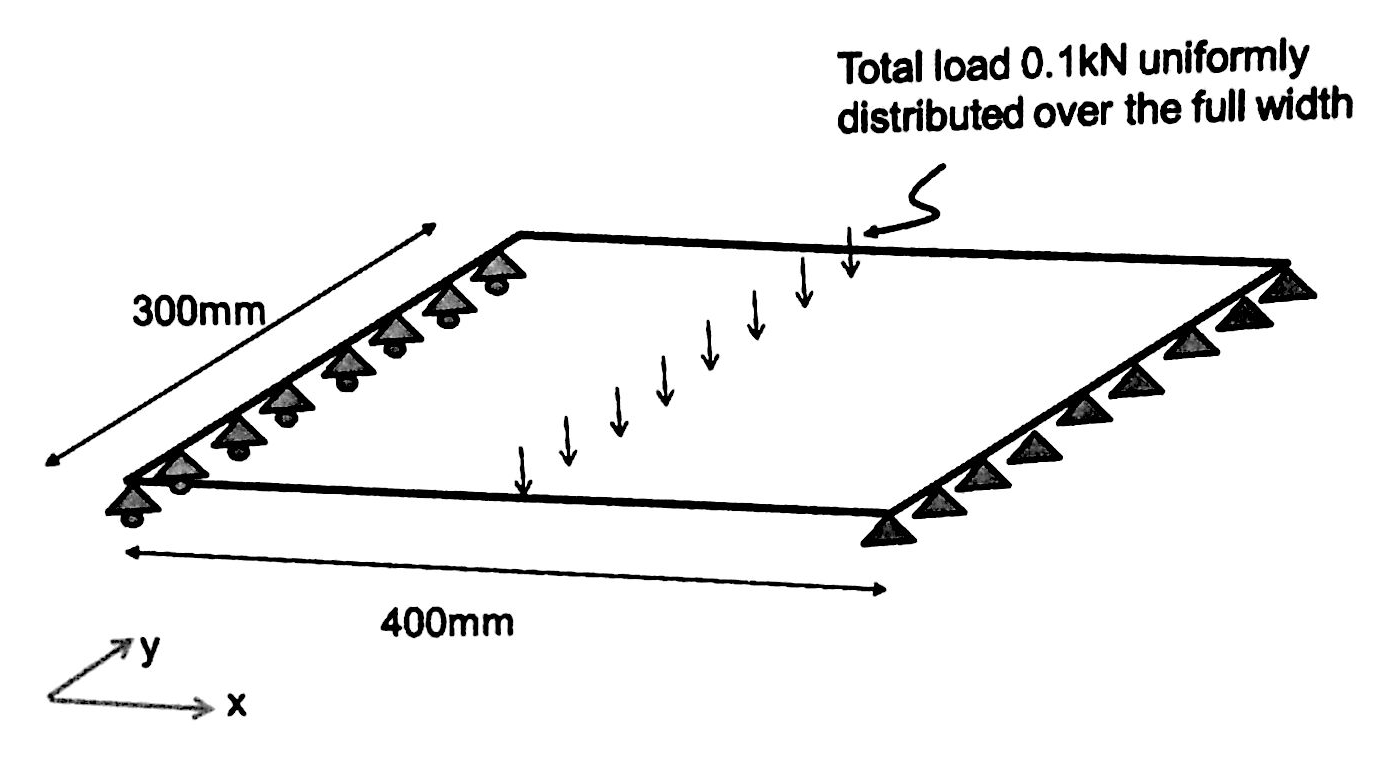
\includegraphics[width=0.7\textwidth]{fig1.png}
\end{center}

\subsection{Laminate Stiffness and Maximum Deflection (Part a)}

\textit{Use laminate analysis to compute the relevant laminate stiffnesses and classical
beam bending formulae to estimate maximum deflection at the center of the
plate.}
%
\\The input for the \emph{Laminate Analysis Program} are the values obtained in
the first part, and entered to the program as given below.
%
\begin{center}
  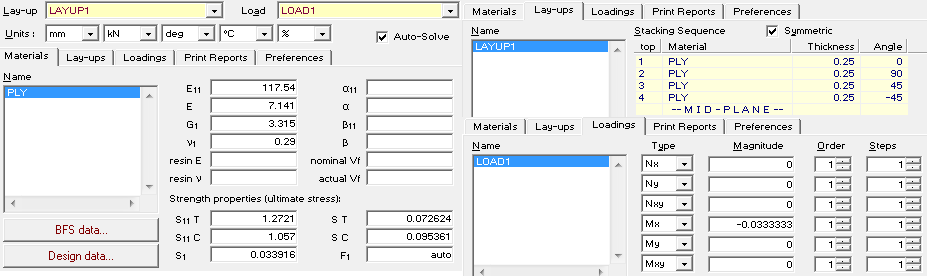
\includegraphics[width=\textwidth]{laminate2.png}
\end{center}
%
For the given input, the program yields the following laminate stiffnesses.
%
\begin{center}
  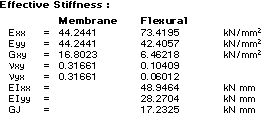
\includegraphics{laminate1.png}
\end{center}
%
As for the classical beam bending solution,

\begin{equation}
  \delta_{\max} = \delta_B + \delta_S = \frac{1}{48}\frac{PL^3}{EI} + \frac{1}{4} \frac{PL}{GA}
\end{equation}
%
where $P=\SI{0.1}{kN}$, $E = \SI{73.4195}{GPa}$, $G=\SI{6.46218}{GPa}$,
$I = \frac{1}{12} b h^3 = \SI{200}{mm^4}$, $A=\SI{600}{mm^2}$ with $b =
\SI{300}{mm}$, $h = 8 \times 0.25 = \SI{2}{mm}$ and $L=\SI{400}{mm}$.
%
\\Substituting the values, one obtains
%
\begin{equation}
  \delta_{\max} = \num{9.08024e-3} + \num{25.7911e-6} = \SI{9.10603e-3}{mm}
\end{equation}
%
For the maximum deflection at the center of the plate.

\subsection{First and Last Ply Failure Loads (Part b)}

\textit{Use laminate analysis and the failure data from question 1, to estimate the
first and last ply failure loads.}

The method that was used to determine the failure procedure is this: The indices
were observed at each step of the failure. Since the ply with the highest
index is the most critical one, that one was removed from the model, making it
ready for the next step. This was done until only one ply is standing,
effectively yielding the order of failure and the loads of failure for each
ply.

This can be observed in Figure~\ref{fig:indices1}. According to the figure, the
order of failure is 8 > 6 > 5 > 4 > 7 > 3 > 2 > 1. From the figure, the failing
indices for the first and last plies are respectively 0.075 and 3.0.

Therefore, the first ply failure load (for ply 8) is $0.1/0.075 \approx
\SI{1.333}{kN}$
and last ply failure load (for ply 1) is $0.1/3 = \SI{0.0333}{kN}$

\begin{figure}[H]
\begin{center}
  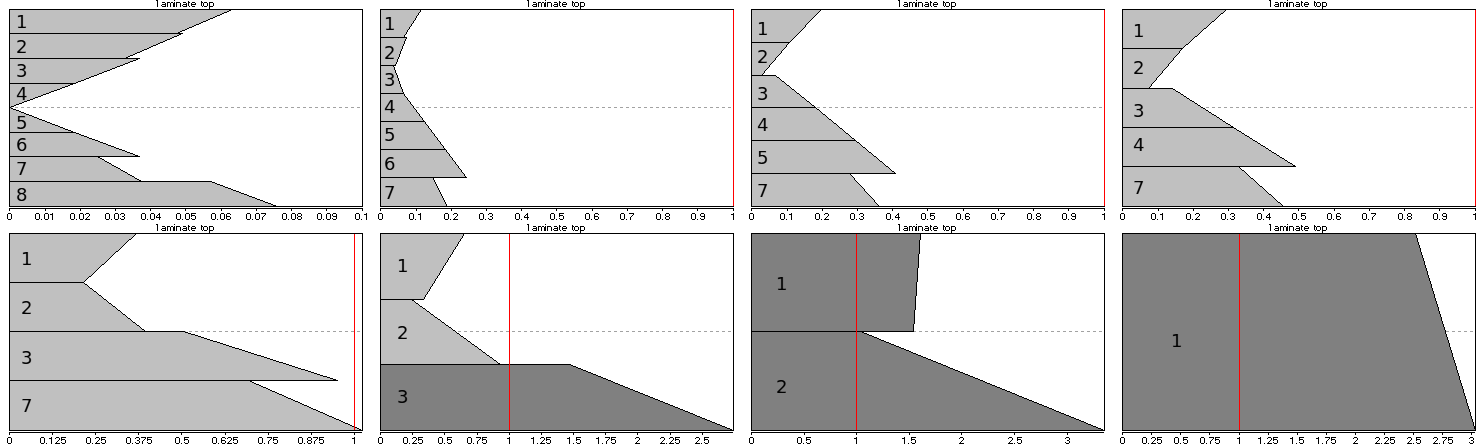
\includegraphics[width=\textwidth]{indices.png}
\end{center}
\caption{The indices for each step of the failure, consecutively from left to
  right, continuing the same way from the second row. Numbers show the remaining
  plies. Numbering denotes the topmost ply as 1 and bottom-most ply as 8}
\label{fig:indices1}
\end{figure}

\section{FEM Model (Task 3)}

\textit{Create a Finite Element model of the above problem having identical
boundary conditions, loadings and material properties.
\\Perform an implicit Finite Element analysis and compute the central
deflection. Compare results with the previous classical solution using laminate
analysis.}

\section{FEM Model with Beads (Task 4)}

\textit{Modify the above finite element model to include two geometric stiffeners (so
called Beads or Sikkens). Choose a suitable spacing for the sickens with each
one having approximate dimensions of 250mm length and 30mm with (15mm height).
Note a useful option exists in Visual Mesh for this operation (2D > Bead on 2D mesh).
The plate with Sikkens has identical loading (line load across the center) and
boundary conditions identical to question 2.}

\begin{center}
  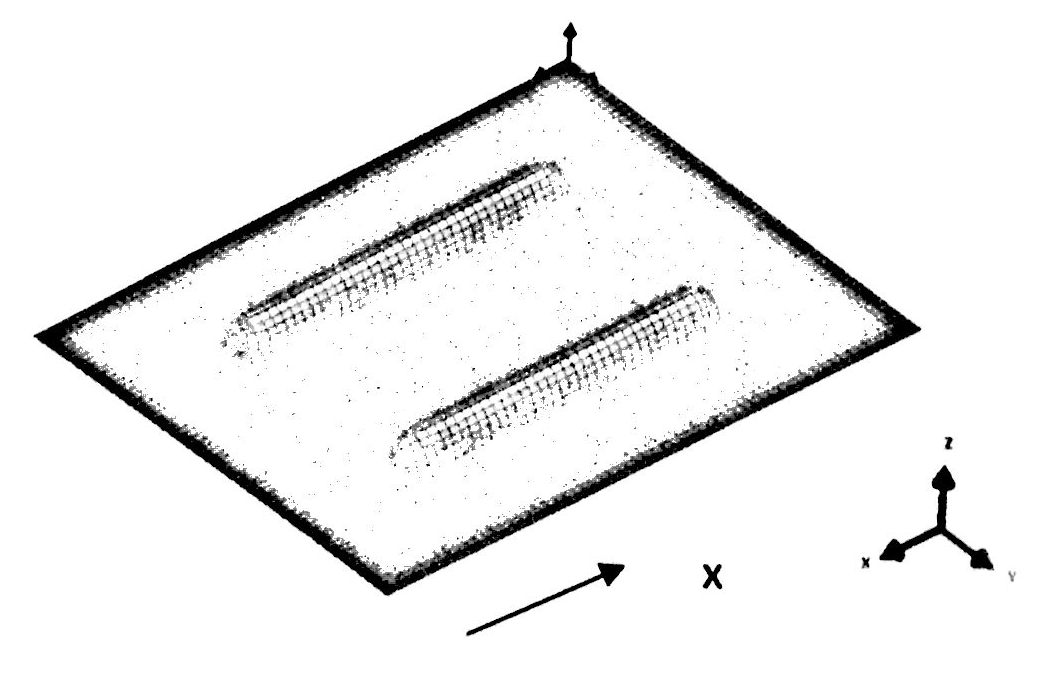
\includegraphics[width=0.7\textwidth]{fig2.png}
\end{center}

\textit{Use the ILAY=1 option to define the laminate, which has the same materials,
lay-up orientations and ply thicknesses as used in questions 2 and 3. Define
Auxiliary 26 to get the failure load indicator for all plies (done in the
material cards). For the output contours to work properly, you will need to use
the ILAY=1 option and also visualize results from the .erfh5 file (for erf5 file
output set ERFKEY=3 in the OCTRL control card).}

\textit{Perform an implicit failure analysis of the plate with Sikkens and compute
\begin{enumerate}
\item The maximum deflection.
\item The failure load using a maximum stress criterion and the composite
  failure data determined from question 1.
\item From the contour results for ``Ply Failure Criteria'' estimate the
  necessary applied load to just cause first ply failure of the structure.
\end{enumerate}}

\section{Resin Infusion (Task 5)}
%
\textit{Perform a PAM-RTM infusion simulation of the Plate with Sikkens.
\\Beware that PAM-RTM uses only triangular shell elements and the units should
be in meters, if you want to be consistent with default data provided in
PAM-RTM. Both element type (option MESH > TRANSFORM > SPLIT QUADS...) and units
(option MESH > TRANSFORM > SCALE...) can be converted in PAM-RTM, or in Visual
Mesh with similar options.
\\Assume the resin inlet is as shown below. Use pressure injection with 1 bar
difference between inlet and outlet. Assume the infusion is isothermal at room
temperature and the fabric has isotropic permeability throughout.}
%
\begin{table}[H]
  \centering
  \begin{tabular}{ll}
    \toprule
    Thickness of composite & 2 mm\\
    Resin viscosity at 23\degree C & 0.3 Pa sec \\
    Assume PAM-RTM standard fabric with porosity & 0.5 \\
    Fabric permeability & \num{1e-10} m\textsuperscript{2}\\
    \bottomrule
  \end{tabular}
  \caption{Infusion and other data}
\end{table}
%
\begin{center}
  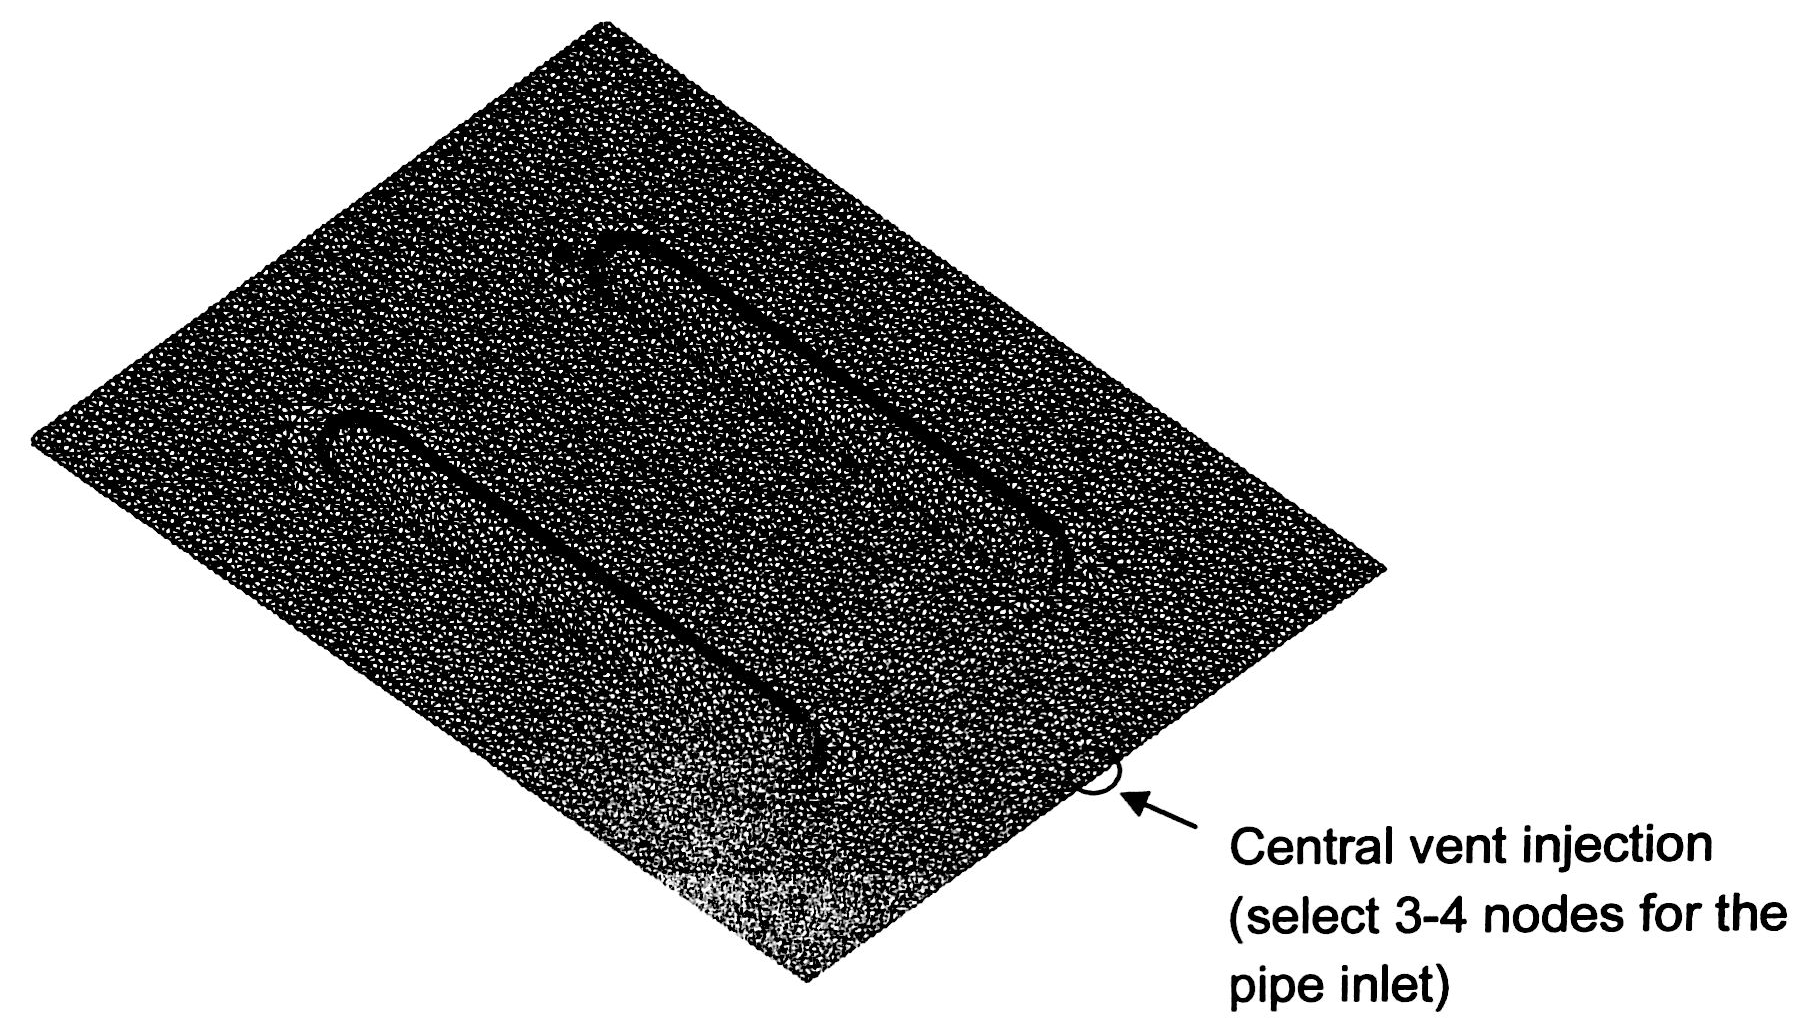
\includegraphics[width=0.7\textwidth]{fig3.png}
\end{center}
%
\textit{Perform an RTM type analysis and estimate:
%
\begin{enumerate}
\item The time for infusion and suitable positions for the outlet vents.
\item If the resin is known to gel after 30 minutes, is the infusion likely to
  be successful?
\item Propose and try an alternative infusion strategy with a view to speeding
  up the infusion time and having a good infusion. Where should the outlet vents
  be placed for your chosen setup?
\end{enumerate}}

As can be seen from Figure~\ref{fig:resin1}, numerous simulations have been done
with PAM--RTM using different resin inlets.

For the proposed setting in the first part, the inlets and outlets have been
placed as shown under the upper-left plot in Figure~\ref{fig:resin1}, i.e.
outlets in the middle and corners opposite to the inlet.
This has been done to ensure a pressure gradient suitable for the infusion to
complete. The result of the proposed setting can be observed in the same figure.

The time of the infusion for the
proposed setting is equal to \SI{3220}{s} $\approx$ \SI{54}{min}.
This result is well over the \SI{30}{min} limit given in the second part. Hence
the resin would solidify before the process is complete and the infusion would
be unsuccessful.

For the third part, a number of different configurations have been tried. The
most successful one is the one seen in the lower-right of
Figure~\ref{fig:resin1}, which had a duration of \SI{650}{s} $\approx$
\SI{11}{min}. This configuration, in which the \emph{four inlets are located on the centers
of both opposing edges with an outlet in the middle}, has proven to be the most
effective among all viable configurations which has a realistic amount of
inlets. Of course, one can imagine a system with inlets more than four, or the
whole boundary is an inlet; but I presumed it would be logical
to remain in realistic ranges, which in this case is four inlets maximum.

Another issue to address is the unreliability of the suggested software. The
question has stated that 3--4 nodes be used for the pipe inlet, however these
facts exist for the case: A minimum number of 2 nodes can be selected for a
pipe inlet, which leads me to believe the program uses a naive algorithm that
takes line elements as input. After 2 nodes, the infusion duration decreases by
\%20 with every extra node added to the inlet. This means that the results
should have an error margin of at least \%20. Additionally, adding outlets to
the case had no effect on the simulation, and the resin continued to flow the
same way without them. This has led me to believe it is not the pressure
gradient that sets the resin into motion, but some other criterion inside the
program.
Nevertheless, it is not my duty
to question the internal mechanism of the program and I shall finish this
paragraph knowing that I have stated my concerns.

\begin{figure}[H]
\begin{center}
  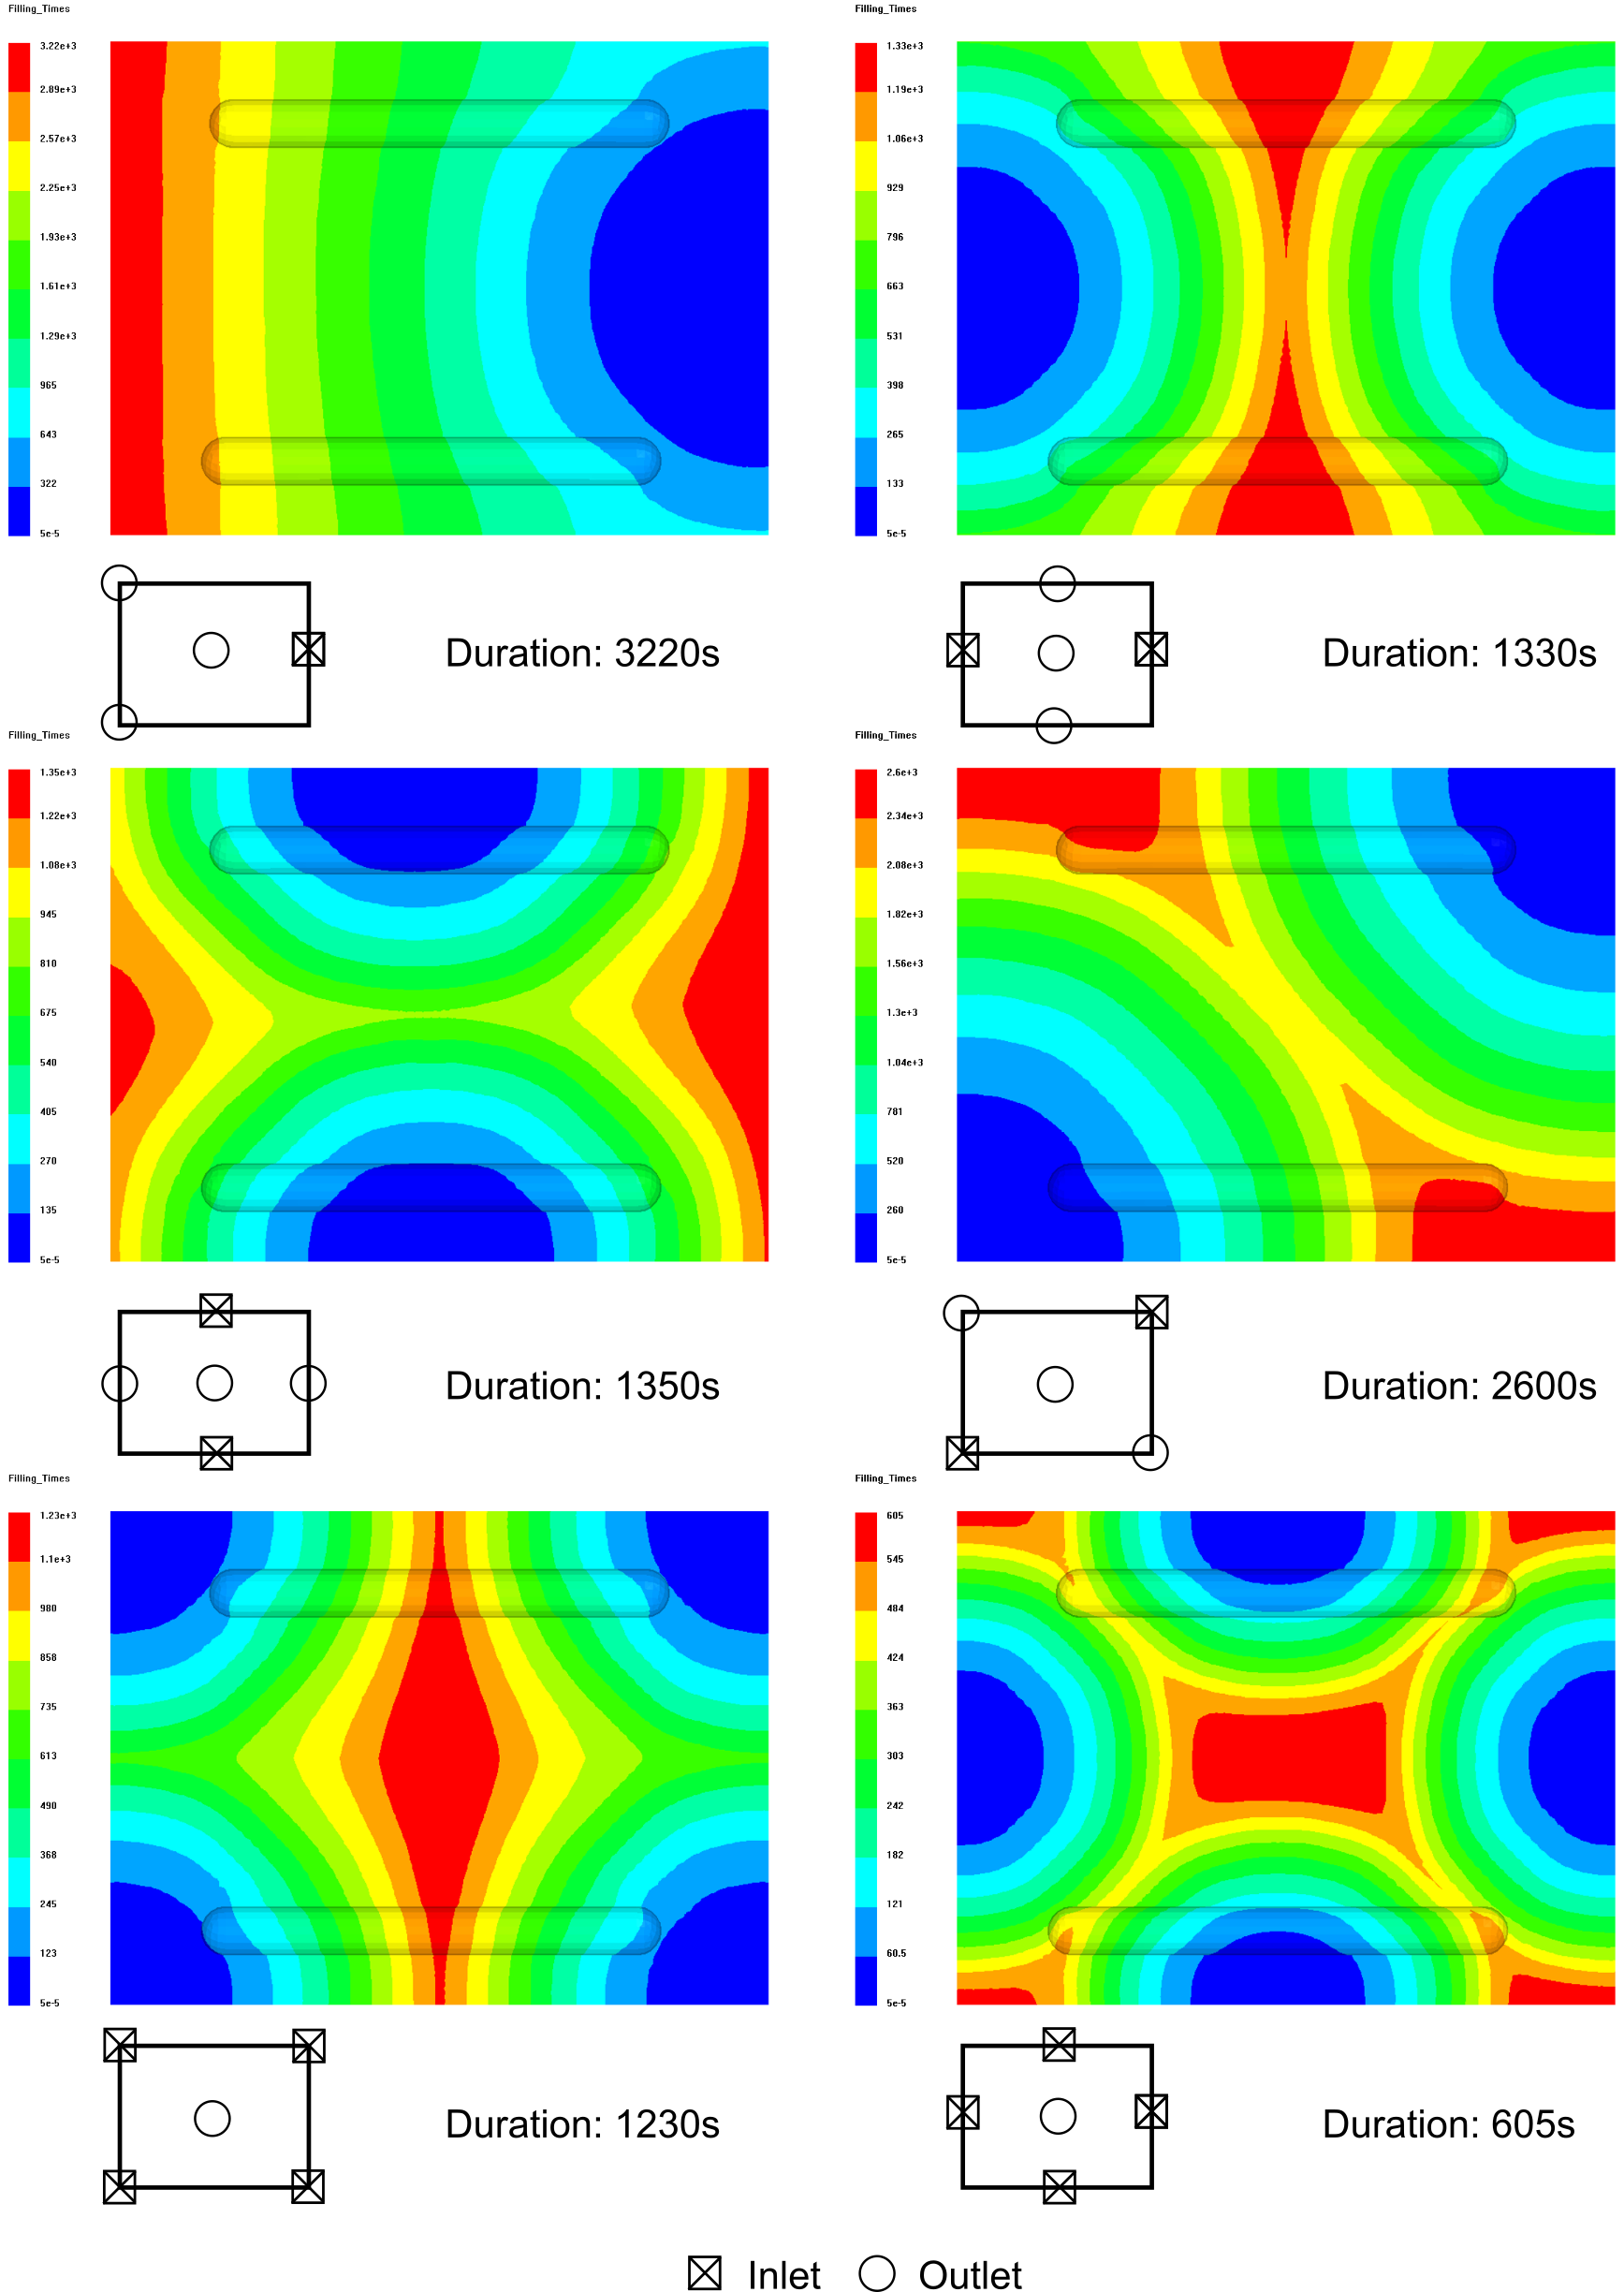
\includegraphics[width=16cm]{q5.png}
\end{center}
\caption{The color plots show the progression of the resin over time, with blue
  showing the starting region, hence the inlets, and red showing the last region
  to be infused. Under every plot is a diagram showing the locations of the
  inlets, outlets and the duration of the infusion. The symbols have been
  explained at the bottom of the figure.}
\label{fig:resin1}
\end{figure}

\section{Discussion and Conclusion}

\end{document}
%
